%% 
%% ACS project dissertation template. 
%% 
%% Currently designed for printing two-sided, but if you prefer to 
%% print single-sided just remove ",twoside,openright" from the 
%% \documentclass[] line below. 
%%
%%
%%   SMH, May 2010. 

\documentclass[a4paper,12pt,twoside,openright]{report}
\usepackage{graphicx}

%%
%% EDIT THE BELOW TO CUSTOMIZE
%%

\def\authorname{Martin Marinov\xspace}
\def\authorcollege{St Edmund's College\xspace}
\def\authoremail{mtm46@cam.ac.uk}
\def\dissertationtitle{Remote Video Eavesdropping Using a Software Defined Radio Platform}
\def\wordcount{??,???}


\usepackage{epsfig,graphicx,parskip,setspace,tabularx,xspace,epstopdf} 
\graphicspath{ {./images/} }

%% START OF DOCUMENT
\begin{document}


%% FRONTMATTER (TITLE PAGE, DECLARATION, ABSTRACT, ETC) 
\pagestyle{empty}
\singlespacing
% title page information
\begin{titlepage} 

\begin{center}
\noindent
\huge
\dissertationtitle \\
\vspace*{\stretch{1}}
\end{center}

\begin{center}
\noindent
\huge
\authorname \\
\Large
\authorcollege      \\[24pt]

\includegraphics{CUni3.eps}
\end{center}

\vspace{24pt} 

\begin{center}
\noindent
\large
{\it A dissertation submitted to the University of Cambridge \\ 
in partial fulfilment of the requirements for the degree of \\ 
Master of Philosophy in Advanced Computer Science} 
\vspace*{\stretch{1}}
\end{center}

\begin{center}
\noindent
University of Cambridge \\
Computer Laboratory     \\
William Gates Building  \\
15 JJ Thomson Avenue    \\
Cambridge CB3 0FD       \\
{\sc United Kingdom}    \\
\end{center}

\begin{center}
\noindent
Email: \authoremail \\
\end{center}

\begin{center}
\noindent
\today
\end{center}

\end{titlepage} 

\newpage
\vspace*{\fill}

\onehalfspacing
\newpage
{\Huge \bf Declaration}

\vspace{24pt} 

I \authorname of \authorcollege, being a candidate for the M.Phil in
Advanced Computer Science, hereby declare that this report and the
work described in it are my own work, unaided except as may be
specified below, and that the report does not contain material that
has already been used to any substantial extent for a comparable
purpose.

\vspace{24pt}
Total word count: \wordcount

\vspace{60pt}
\textbf{Signed}: 

\vspace{12pt}
\textbf{Date}:


\vfill

This dissertation is copyright \copyright 2014 \authorname. 
\\
All trademarks used in this dissertation are hereby acknowledged.



\newpage
\vspace*{\fill}

\singlespacing
\newpage
{\Huge \bf Abstract}
\vspace{24pt} 


This dissertation presents a software toolkit for remotely eavesdropping video monitors using a Software Defined Radio (SDR) receiver. It exploits compromising emanations from cables carrying video signals. Analogue video is usually transmitted one line of pixels at a time encoded as a varying current. This generates a wideband electromagnetic wave that can be picked up by an SDR receiver. The presented software can map the received field strength of each pixel to a grayscale value in order to show a real-time false colour estimate of the original video signal.

The software significantly lowers the costs required for undertaking a practical attack compared to existing solutions. Furthermore, it allows for an additional digital post-processing which can aid in analysing and improving the results. It also provides mobility for a potential adversary, requiring only a commodity laptop and an USB SDR dongle. The attacker does not need to have any prior knowledge about the victim's video display. All parameters such as resolution and refresh rate can be estimated with the aid of the software. 

The software comprises of a library written in C, a collection of plug-ins for various Software Define Radio (SDR) frontends and a Java based Graphical User Interface (GUI). It is designed to be a multi-platform application. All native libraries can be pre-compiled and packed into a single Java jar file which allows the toolkit to run on any supported operating system.

This report documents the digital processing techniques that have been employed in order to extract, detect and lock to a video signal. It also explains the architecture of the software system and the techniques used in order to achieve low latency and real-time interactivity. It demonstrates the usage of the system by performing a practical attack. It then gives some ideas about what could be improved further and some analysis of data that was collected during the development of the software.


\newpage
\vspace*{\fill}


\pagenumbering{roman}
\setcounter{page}{0}
\pagestyle{plain}
\tableofcontents
%% \listoffigures
%% \listoftables

\onehalfspacing

%% START OF MAIN TEXT 

\chapter{Introduction}
\pagenumbering{arabic} 
\setcounter{page}{1} 

\section{Related Work} 

[Related work and critique]

\section{Availability} 
[Github repo url]

\cite{kuhn2003compromising}

\chapter{Background}

\section{Electronic Emanations} 

\section{IQ sampling} 

\chapter{Methodology} 

[Explain how the whole system works in high level]

[TODO! Explain how resolution and framerate detection works]



\section{Sampling Rate}

[TODO! Explain how bandwidth relates to resolution width * height * framerate = samplerate ]

The sampling rate

\begin{figure}[h!]
  \caption{The original image}
  \centering
    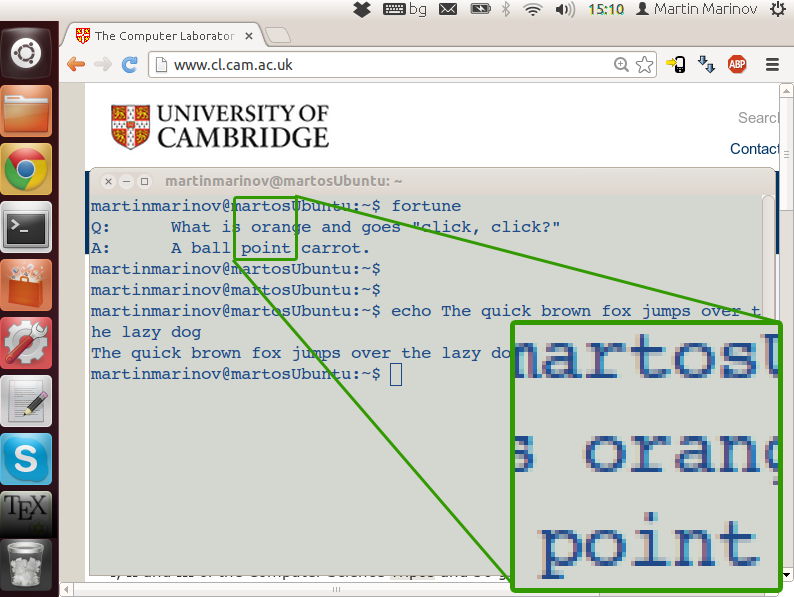
\includegraphics[width=0.5\textwidth]{sr_original}
\end{figure}

\begin{figure}[h!]
\minipage{0.49\textwidth}
  \centering
    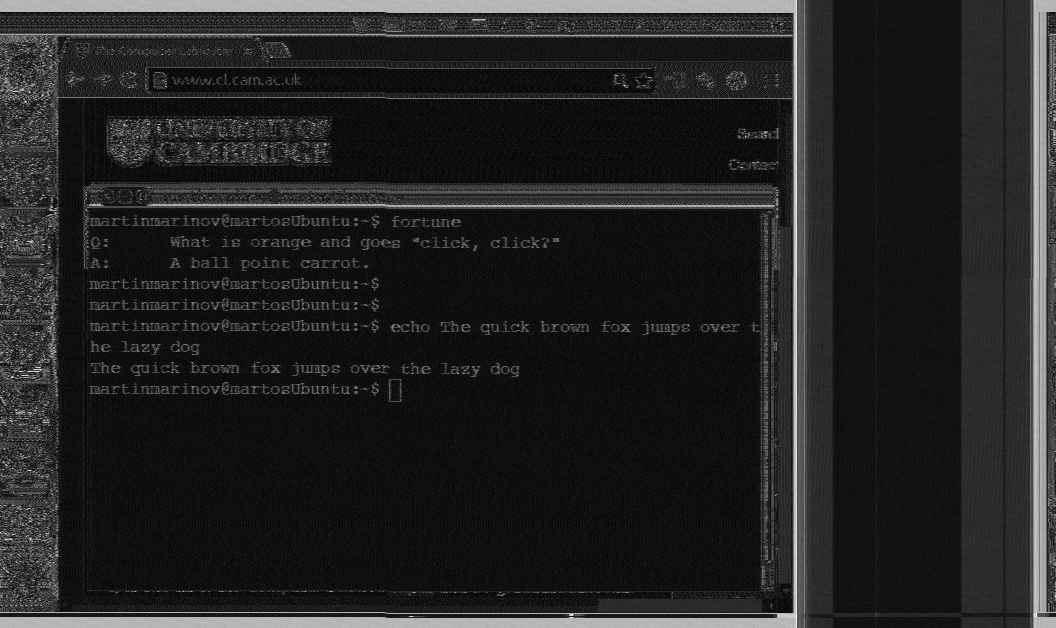
\includegraphics[width=\linewidth]{sr_50MHz_at_190MHz}
  \caption{50 MHz}
\endminipage\hfill
\minipage{0.49\textwidth}
  \centering
    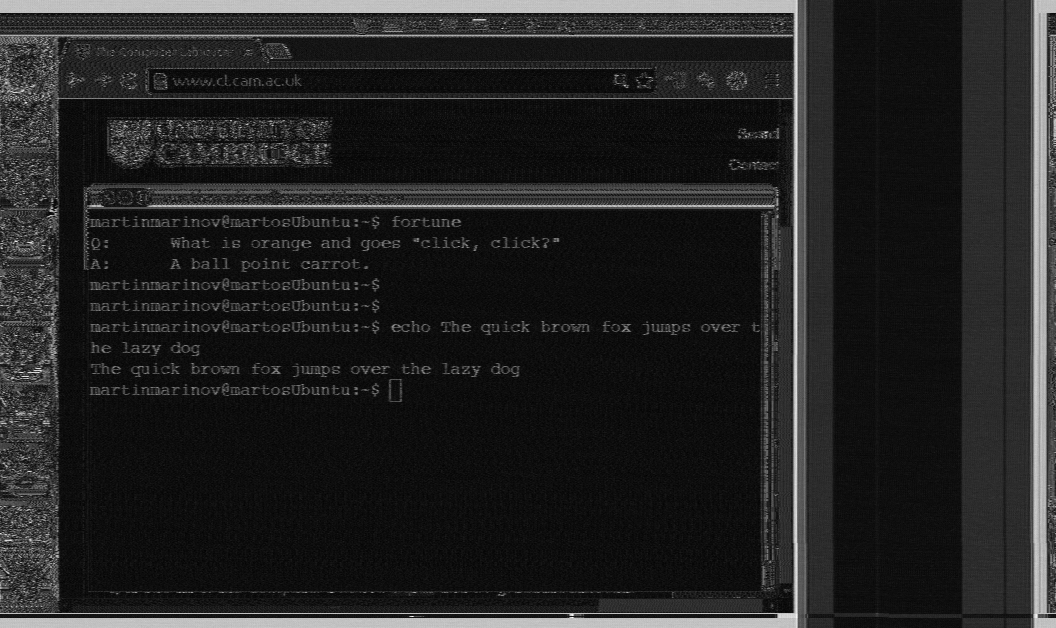
\includegraphics[width=\linewidth]{sr_40MHz_at_190MHz}
  \caption{40 MHz}
\endminipage\hfill
\minipage{0.49\textwidth}
  \centering
    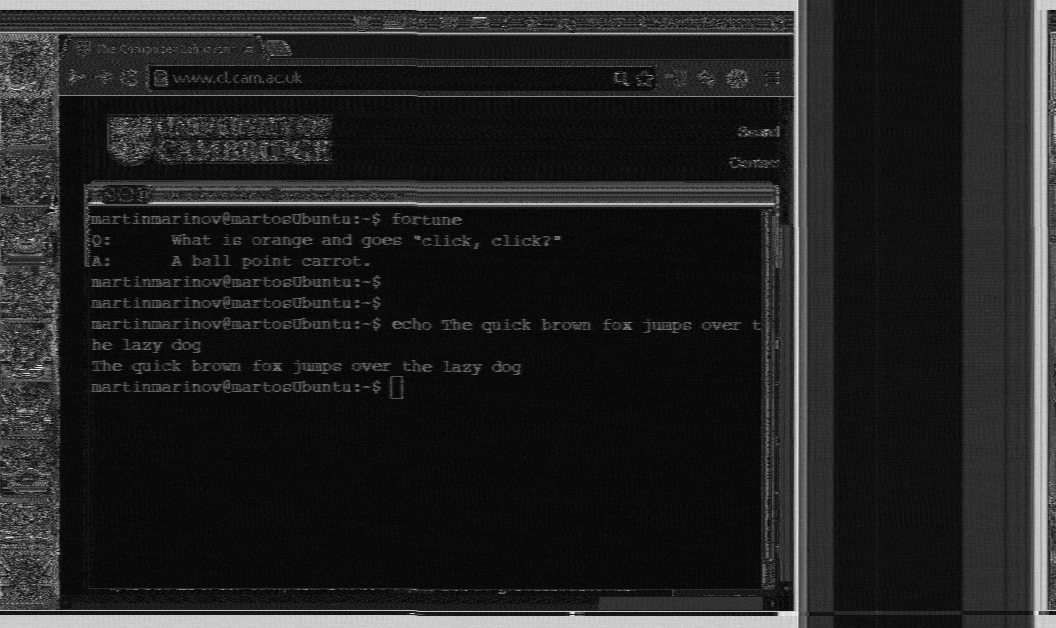
\includegraphics[width=\linewidth]{sr_30MHz_at_190MHz}
  \caption{30 MHz}
\endminipage\hfill
\minipage{0.49\textwidth}
  \centering
    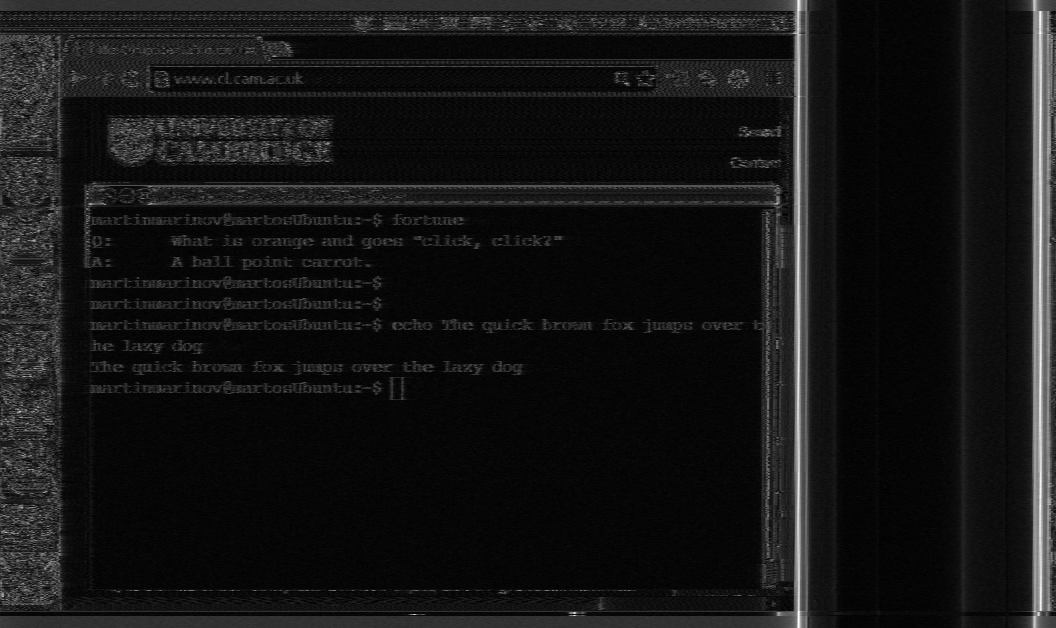
\includegraphics[width=\linewidth]{sr_20MHz_at_190MHz}
  \caption{20 MHz}
\endminipage\hfill
\minipage{0.49\textwidth}
  \centering
    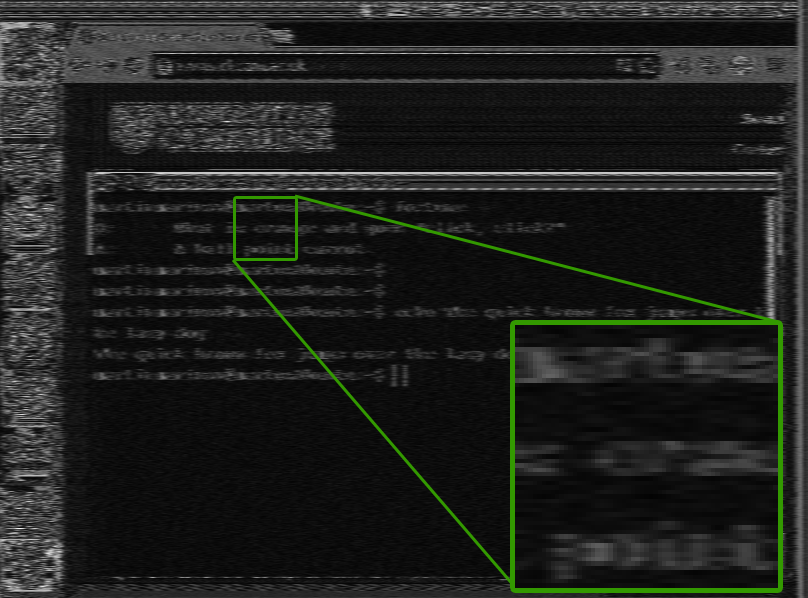
\includegraphics[width=\linewidth]{sr_10MHz_at_190MHz}
  \caption{10 MHz}
\endminipage\hfill
\minipage{0.49\textwidth}
  \centering
    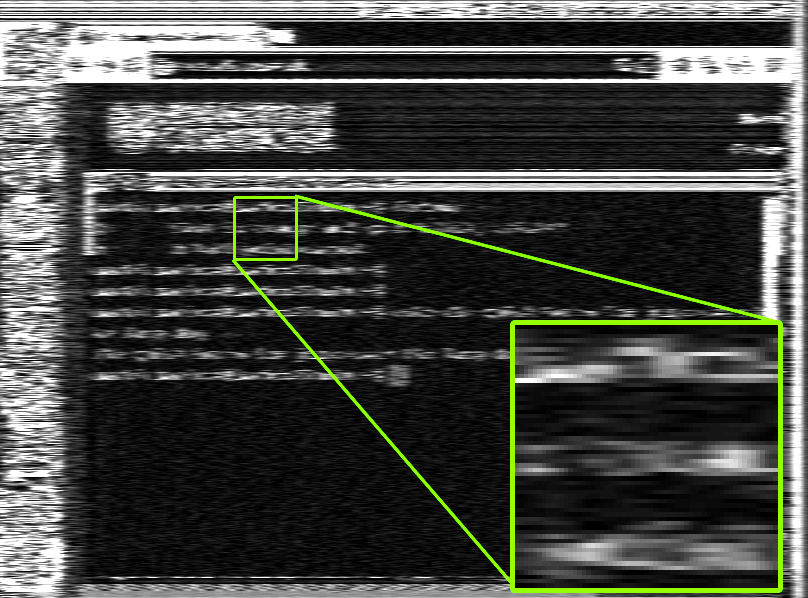
\includegraphics[width=\linewidth]{sr_5MHz_at_190MHz}
  \caption{5 MHz}
\endminipage
\end{figure}


\chapter{Practical attack} 

Before explaining how the software works internally, let's present a demonstration of a practical video eavesdropping attack. Its main aim is to show the ease with which such an attack could happen. In the meantime this will give an opportunity to explain the characteristics of the received signal and how they are exploited.

As in the real world, we will start with no knowledge of the victim's system. We will estimate the frequency at which the emission strength has the best Signal to Noise Ratio (SNR). We will then analyse the signal to detect the resolution and refresh rate of the screen. We will afterwards lock onto the signal and try to recover the original video. We will also discuss some techniques that could be utilized to improve the quality of the image.

\section{The Setup}

The choice for a SDR front-end for this demonstration is a USRP B200\footnote{Refer to \ref{sec:hw} Hardware for discussion on currently available SDR devices.}. Depending on the particular requirements, an attacker might prefer mobility over accuracy and choose the smaller FlexiTV\texttrademark MSi3101 SDR USB Dongle. However, for this demonstration we will attempt to obtain the highest possible resolution. Therefore we need an SDR radio that is capable of obtaining a wide bandwidth. This makes the 32 MHz of Bandwidth that the USRP provides a much better choice than the 8 MHz available from the Mirics dongle.

[Antenna]

[Location of victim]

[Victim's fonts]

\section{Preparation}

\chapter{Implementation} 

\section{Hardware}
\label{sec:hw} 

\section{Architecture}

\subsection{Main Library}

\subsection{JavaGUI}

\subsubsection{Multiplatform}

\subsubsection{Graphical Interface}

\subsubsection{Visualisation}

\section{Digital Signal Processing}

\subsection{Overview}

\subsection{Signal Reconstruction}

\subsubsection{Multithreading}

\subsubsection{Demodulation}

\subsubsection{Re-sampling}

\subsubsection{Auto Gain}

\subsubsection{Low-pass}

\subsection{Frame Synchronization}

\subsection{Resolution Detection}

\subsection{Extended Bandwidth}

\subsection{Testing and Benchmarking}

\chapter{Summary and Conclusions} 

[Summarize results]

[potential future work]

\appendix
\singlespacing

\bibliographystyle{unsrt} 
\bibliography{dissertation} 

\end{document}
